% The contents of this file is 
% Copyright (c) 2009-  Charles R. Severance, All Righs Reserved

\chapter{Programas conectados por uma rede}

Enquanto que muitos dos exemplos usados neste livro tem focado na leitura
de arquivos e a procura por dados nesses arquivos, existem muitas fontes
de informação diferentes quando se leva em conta a Internet.

Nesse capítulo nós iremos fingir ser um navegador web e obter páginas
web usando o HyperText Transport Protocol (HTTP), em português Protocolo
de Transferência de Hipertexto.  Feito isso, nós iremos fazer uma leitura
pelos dados da página web e analisá-los.

\section{Protocolo de Transferência de Hipertexto - HTTP na sigla em inglês}

O protocolo de rede que impulsiona a web é, na verdade, bem simples e 
existe um suporte embutido no Python chamado {\tt sockets} que faz com seja
muito fácil estabelecer conexões de rede e obter dados através desses
sockets com um programa Python.

Um {\bf socket} é bem parecido com um arquivo, exceto que um único socket 
provê uma conexão de duas vias entre dois programas.  Você pode tanto ler
quanto escrever pelo mesmo socket.  Se você escrever alguma coisa em um
socket, a escrita é enviada para a aplicação na outra ponta do socket.
Se você ler a partir de um socket, você está recebendo os dados que a outra
aplicação está enviando.

Mas se você tentar ler um socket enquanto que o programa na outra ponta do
socket não envia nenhum dado---você tem que sentar e esperar.  Se os
programas de ambos os lados do socket simplesmente esperarem por dados sem
enviarem nada, eles irão esperar por muito tempo.

Então, uma parte importante de programas que se comunicam através da Internet
é ter algum tipo de protocolo.  Um protocolo é um conjunto de regras precisas
que determinam quem inicia, como é o relacionamento, e então quais são as
respostas para a mensagem enviada, e quem envia a próxima. E assim por diante.
Em certo sentido, como duas aplicações, cada uma em uma ponta do socket, vão
dançar e garantir que uma não vair pisar no pé da outra.

Existem muitos documentos que descrevem esses protocolos de rede.  O Protocolo
de Transferência de Hipertexto descrito no seguinte documento:

\url{http://www.w3.org/Protocols/rfc2616/rfc2616.txt}

Este é um longo e complexo documento de 176 páginas, com muitos detalhes.  Se
você achar ele interessante, fique à vontade para lê-lo na integra.  Mas se
você der uma olhada pela página 36 do RFC2616, você irá encontrar a sintaxe
para a requisição GET.  Para requerer um documento de um servidor web, nós
fazemos uma conexão com o servidor {\tt www.py4inf.com} na porta 80, e então
enviamos uma linha com formato

{\tt GET http://www.py4inf.com/code/romeo.txt HTTP/1.0 }

onde o segundo parâmetro é a página web que nós estamos solicitando, e então
nós também enviamos uma linha em branco.  O servidor web irá responder com
alguma informação de cabeçalho sobre o documento e uma linha em branco seguida
do conteúdo do documento.

\section{O Navegador Web Mais Simples do Mundo}

Talvez, a maneira mais simples de mostrar como o protocolo HTTP funciona é
escrever um programa Python bem simples que faz a conexão com um servidor web
e segue as regras do protocolo HTTP para solicitar um documento e exibir o
que o servidor envia de volta.

\beforeverb
\begin{verbatim}
import socket

mysock = socket.socket(socket.AF_INET, socket.SOCK_STREAM)
mysock.connect(('www.py4inf.com', 80))
mysock.send('GET http://www.py4inf.com/code/romeo.txt HTTP/1.0\n\n')

while True:
    data = mysock.recv(512)
    if ( len(data) < 1 ) :
        break
    print data

mysock.close()
\end{verbatim}
\afterverb
%
Primeiro o programa estabelece a conexão na porta 80 no 
servidor \url{www.py4inf.com}.
Como nosso programa faz o papel de um ``navegador web'', o protocolo HTTP
informa que nós temos que enviar um comando GET seguido de uma linha em branco.

\beforefig
\centerline{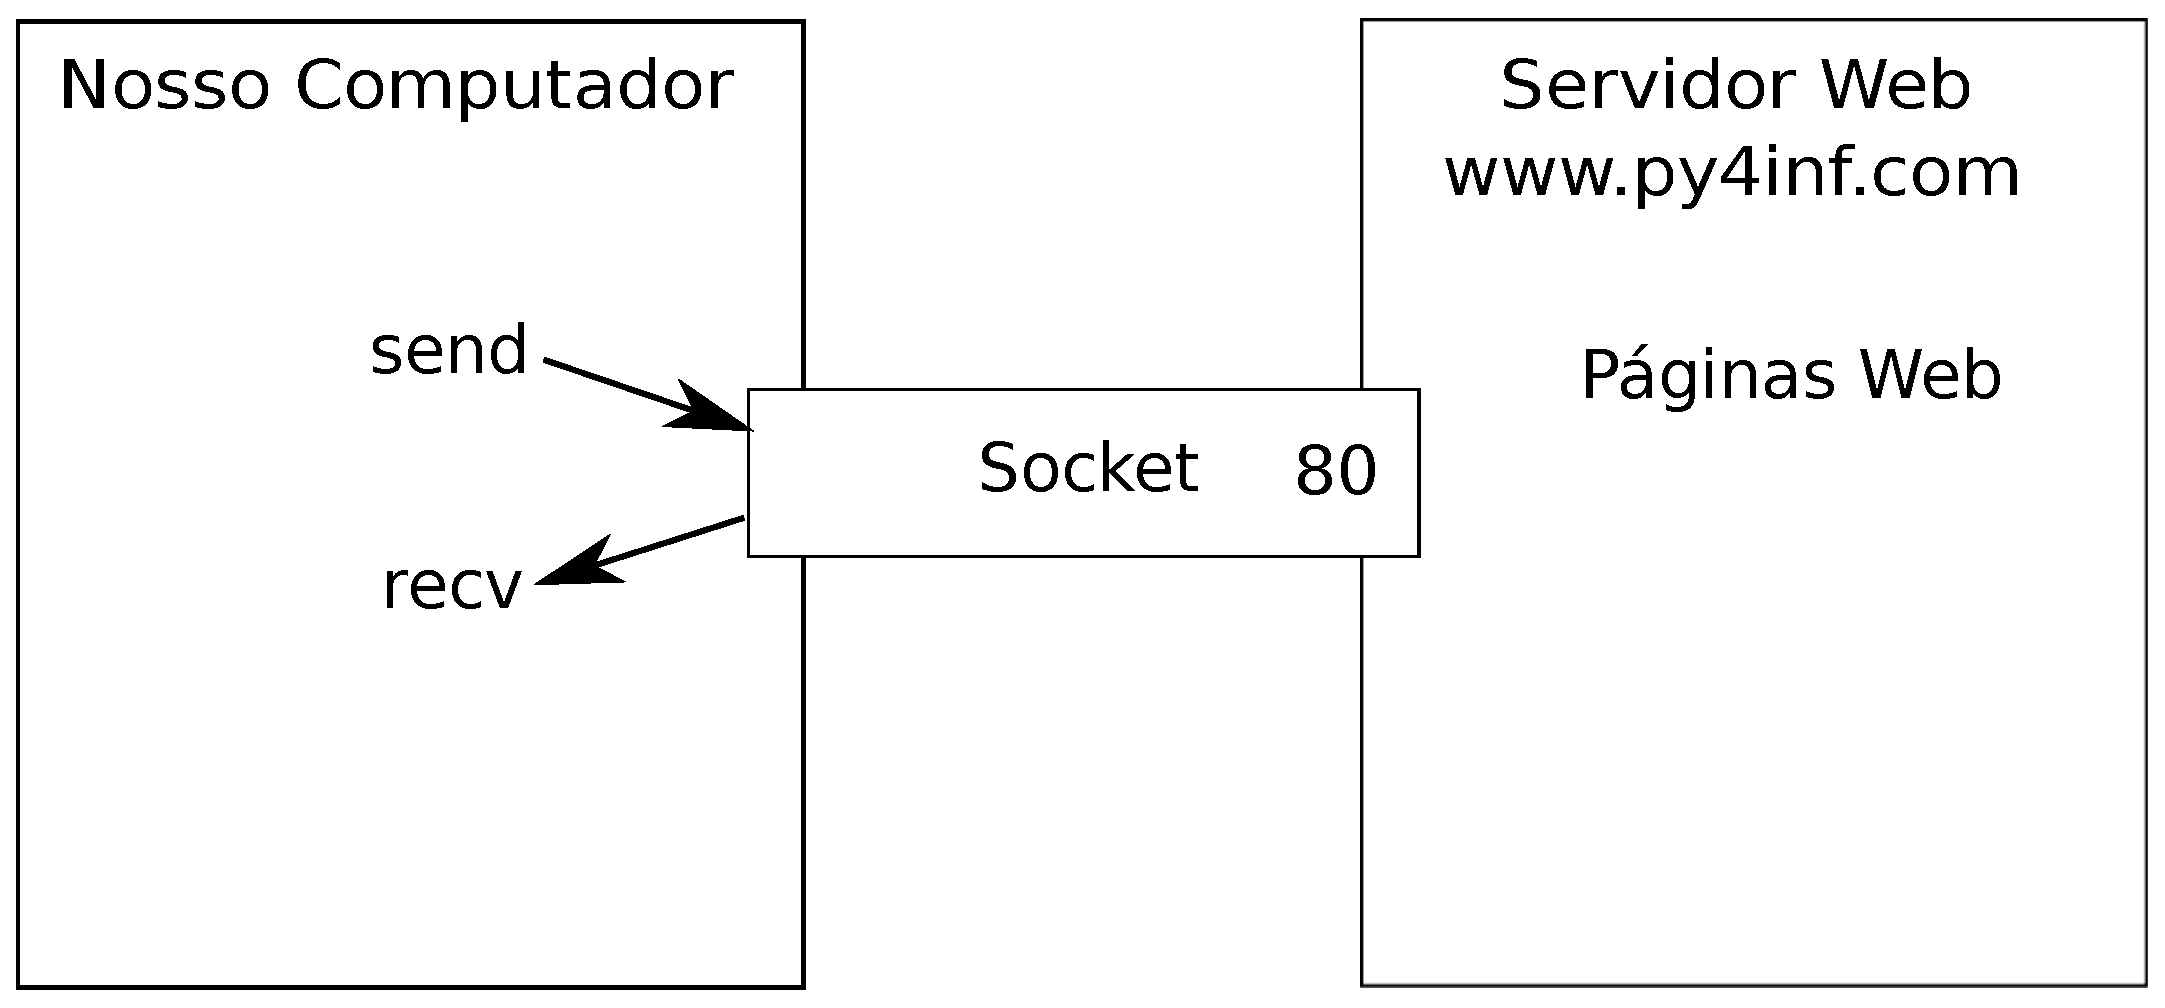
\includegraphics[height=1.50in]{figs2/socket.eps}}
\afterfig

Uma vez enviada a linha em branco, nós escrevemos um loop que recebe do
socket dados em pedaços de 512 caracteres e imprime os dados até que não
exista mais dados para ler (por exemplo, a recv() retorna uma string vazia).

O programa produz a seguinte saída:

\beforeverb
\begin{verbatim}
HTTP/1.1 200 OK
Date: Sun, 14 Mar 2010 23:52:41 GMT
Server: Apache
Last-Modified: Tue, 29 Dec 2009 01:31:22 GMT
ETag: "143c1b33-a7-4b395bea"
Accept-Ranges: bytes
Content-Length: 167
Connection: close
Content-Type: text/plain

But soft what light through yonder window breaks
It is the east and Juliet is the sun
Arise fair sun and kill the envious moon
Who is already sick and pale with grief
\end{verbatim}
\afterverb
%
A saída começa com os cabeçalhos que o servidor web envia
para descrever o documento.
Por exemplo, o cabeçalho {\tt Content-Type} indica que
o documento é um documento em texto plano ({\tt text/plain}).

Depois que o servidor nos enviar os cabeçalhos, ele adiciona uma
linha em branco para indicar o final dos cabeçalhos, e então, envia
realmente os dados do arquivo {\tt romeo.txt}.

Esse exemplo mostra como fazer uma conexão de rede de baixo nível
com sockets.   Sockets podem ser usados para se comunicar com um
servidor web ou com um servidor de email ou muitos outros tipos
de servidores. Tudo que é preciso é encontrar o documento que
descreve o protocolo e escrever o código para enviar e receber os 
dados de acordo com o protocolo.

Contudo, como o protocolo que nós mais comumente usamos é
o protocolo web HTTP, o Python tem uma biblioteca especificamente
desenvolvida para ter suporte ao protocolo HTTP. E assim, obter 
documentos e dados através da web.

\section{Obtendo uma imagem através do HTTP}

\index{urllib!image}
\index{image!jpg}
\index{jpg}
No exemplo acima, nós pegamos um arquivo em texto plano 
que tinha nova linhas dentro do arquivo e nós simplesmente
copiamos os dados para a tela a medida que o programa era
executado.   Nós podemos usar um programa similar para
obter uma imagem através da web usando o HTTP.   Ao invés de
copiar os dados para a tela, a medida que o programa é
executado, nós acumulamos os dados em uma string, retiramos
os cabeçalhos, e então salvamos os dados da imagem em um
arquivo. Como a seguir:

\beforeverb
\begin{verbatim}
import socket
import time

mysock = socket.socket(socket.AF_INET, socket.SOCK_STREAM)
mysock.connect(('www.py4inf.com', 80))
mysock.send('GET http://www.py4inf.com/cover.jpg HTTP/1.0\n\n')


count = 0
picture = "";
while True:
    data = mysock.recv(5120)
    if ( len(data) < 1 ) : break
    # time.sleep(0.25)
    count = count + len(data)
    print len(data),count
    picture = picture + data

mysock.close()

# Look for the end of the header (2 CRLF)
pos = picture.find("\r\n\r\n");
print 'Header length',pos
print picture[:pos]

# Skip past the header and save the picture data
picture = picture[pos+4:]
fhand = open("stuff.jpg","wb")
fhand.write(picture);
fhand.close()
\end{verbatim}
\afterverb
%
Quando o programa é executado, ele produz a seguinte saída:

\beforeverb
\begin{verbatim}
$ python urljpeg.py 
2920 2920
1460 4380
1460 5840
1460 7300
...
1460 62780
1460 64240
2920 67160
1460 68620
1681 70301
Header length 240
HTTP/1.1 200 OK
Date: Sat, 02 Nov 2013 02:15:07 GMT
Server: Apache
Last-Modified: Sat, 02 Nov 2013 02:01:26 GMT
ETag: "19c141-111a9-4ea280f8354b8"
Accept-Ranges: bytes
Content-Length: 70057
Connection: close
Content-Type: image/jpeg
\end{verbatim}
\afterverb
%
Você pode ver que nesse caso, o cabeçalho 
{\tt Content-Type} indica que o corpo do
documento é uma imagem ({\tt image/jpeg}).
Uma vez terminado o programa, você pode ver os dados da imagem
abrindo o arquivo {\tt stuff.jpg} com um visualizador
de imagems.

Durante a execução do programa, você pode ver que nós não temos
5120 caracteres para cada vez que nós chamamos o método
{\tt recv()}. Nós pegamos tantos caracteres quantos foram
transferidos através da rede, do servidor web para nós, no momemto que
nós chamamos {\tt recv()}.  Neste exemplo, nós pegamos 1460 ou 2920 
caracteres cada vez que nós o solicitamos até chegar a 5120 caracteres
de dados.

Os seus resultados podem ser diferentes, dependendo da velocidade de
sua rede.  Note também que na última chamada de {\tt recv()}, nós pegamos
1681 bytes, que é o final do fluxo (stream), e na chamada seguinte da
{\tt recv()} nós recebemos uma string vazia (zero-length). Que nos informa
que o servidor chamou {\tt close()} no seu final de socket e não existe mais
dados para enviar.

\index{time}
\index{time.sleep}
Nós podemos reduzir nossas sucessivas chamada a {\tt recv()}  descomentando
( tirar o '#') a chamada de {\tt time.sleep()}.  Desta forma, nós esperamos
um quarto de segundo depois de cada chamada, e assim, o servidor pode
``se anteceder'' à nós e enviar mais dados antes de nós chamarmos
{\tt recv()} novamente.  Com esse "atraso", o programa é executado
como a seguir:
\beforeverb
\begin{verbatim}
$ python urljpeg.py 
1460 1460
5120 6580
5120 11700
...
5120 62900
5120 68020
2281 70301
Header length 240
HTTP/1.1 200 OK
Date: Sat, 02 Nov 2013 02:22:04 GMT
Server: Apache
Last-Modified: Sat, 02 Nov 2013 02:01:26 GMT
ETag: "19c141-111a9-4ea280f8354b8"
Accept-Ranges: bytes
Content-Length: 70057
Connection: close
Content-Type: image/jpeg
\end{verbatim}
\afterverb
%
Agora, ao invéz de uma primeira e última chamada a {\tt recv()}, nós agora
pegamos 5120 caracteres cada vez que nós pedimos por novos dados.  

Existe um buffer entre o servidor fazendo solicitações {\tt send()} 
e nossa aplicação fazendo solicitações {\tt recv()}.  Quando nós
executamos o programa com o "atraso" estando ativo, em algum momento
o servidor preenche o buffer no socket e é forçado a fazer uma pausa
até que nosso programa comece a esvaziar o buffer.  A pausa, tanto do
envio quanto do recebimento da aplicação, é chamada ``flow control''
(controle de fluxo).
\index{flow control}

\section{Obtendo páginas web com {\tt urllib}}

Embora nós possamos manualmente enviar e receber dados pelo HTTP 
usando a biblioteca socket, existe uma maneira muito mais simples
de realizar essa tarefa comum em Python pelo uso da biblioteca
{\tt urllib}.

Usando a {\tt urllib}, você pode tratar uma página web
de maneira muito parecida a um arquivo.   Você simplesmente
indica qual página web você gostaria de obter e a
{\tt urllib} lida com todo o protocolo HTTP e detalhes sobre
cabeçalhos.

O código equivalente para ler o arquivo {\tt romeo.txt} a partir
da web usando a {\tt urllib} é como o seguinte:

\beforeverb
\begin{verbatim}
import urllib

fhand = urllib.urlopen('http://www.py4inf.com/code/romeo.txt')
for line in fhand:
   print line.strip()
\end{verbatim}
\afterverb
%
Uma vez que a página web tenha sido aberta com 
{\tt urllib.urlopen}, nós podemos tratá-la
como um arquivo e fazer a leitura usando um loop
{\tt for}.   

Quando o programa é executado, nós apenas vemos na
saída o conteúdo do arquvio.   Os cabeçalhos
continuam sendo enviados, mas o código da {\tt urllib}
consome os cabeçalhos e apenas retorna os dados para
nós.

\beforeverb
\begin{verbatim}
But soft what light through yonder window breaks
It is the east and Juliet is the sun
Arise fair sun and kill the envious moon
Who is already sick and pale with grief
\end{verbatim}
\afterverb
%

Como um exemplo, nós podemos escrever 
um programa para obter os dados de
{\tt romeo.txt} e calcular a frequencia
de cada palavra existente dentro do arquivo como a seguir:

\beforeverb
\begin{verbatim}
import urllib

counts = dict()
fhand = urllib.urlopen('http://www.py4inf.com/code/romeo.txt')
for line in fhand:
    words = line.split()
    for word in words:
        counts[word] = counts.get(word,0) + 1   
print counts
\end{verbatim}
\afterverb
%
Novamente, uma vez que nós abrimos a página web, 
nós podemos fazer a leitura como um arquivo local.

\section{Analizando o HTML e varrendo a web}
\index{web!scraping}
\index{parsing HTML}

Um dos usos comuns da capacidade da {\tt urllib} em Python é 
{\bf varrer} a web.   Varrer a web é quando nós escrevemos um programa
que finge ser um navegador web e obtêm páginas, e então examina os dados
nessas páginas a procura de padrões.

Como um exemplo, um mecanismo de busca como o Google irá olhar os fontes
de uma página web e extrair os links para outras páginas e obter
essas páginas, extrair os links para outras páginas e obter essas
páginas, extrair links e assim por diante.   Usando essa técnica,
o Google {\bf mapeia} seu caminho através de quase todas as páginas
na web.   

O Google também usa a frequencia de links das páginas que ele encontra
para uma página em particular de maneira a medir o quão ``importante'' 
uma página é e em que altura a página de aparecer em seus resultados de
pesquisa.

\section{Analisando o HTML através do uso de expressões regulares}

Uma maneira simples de analisar o HTML é usar expressões regulares, para
repetidamente, buscar por e extrair substrings que coincidam com um
padrão em particular.

Aqui está uma página web simples:

\beforeverb
\begin{verbatim}
<h1>The First Page</h1>
<p>
If you like, you can switch to the
<a href="http://www.dr-chuck.com/page2.htm">
Second Page</a>.
</p>
\end{verbatim}
\afterverb
%
Nós podemos construír um expressão regular bem formada para
identificar e extrair os valores dos links do texto abaixo,
como a seguir:

\beforeverb
\begin{verbatim}
href="http://.+?"
\end{verbatim}
\afterverb
%
Nossa expressão regular procura por strings que iniciam com
``href="http://'', seguida de um ou mais caracteres
(``.+?''), seguida por outra aspas.  O ponto de interrogação 
adicionado ao ``.+?'' indica que a expressão é para coincidir
com um padrão de forma ``não gananciosa'', ao invéz de uma
maneira ``gananciosa''. Um padrão não ganancioso tenta encontrar
a {\em menor} string correspondnte possível e a ganaciosa tenta
encontrar a {\em maior} string correspondente possível.
\index{greedy}
\index{non-greedy}

Nós adicionamos parênteses a nossa expressão regular para indicar
qual parte de nossa string correspondente nós gostariamos de extrair, e
foi produzido o seguinte programa:
\index{regex!parentheses}
\index{parentheses!regular expression}

\beforeverb
\begin{verbatim}
import urllib
import re

url = raw_input('Enter - ')
html = urllib.urlopen(url).read()
links = re.findall('href="(http://.*?)"', html)
for link in links:
    print link
\end{verbatim}
\afterverb
%
O mêtodo de expressão regular {\tt findall} irá retornar para nós uma
lista de todas as strings que coincidem com nossa expressão regular,
retornando apenas o texto do link entre as aspas duplas.

Quando nós executamos o programa, nós temos a seguinte saída:

\beforeverb
\begin{verbatim}
python urlregex.py 
Enter - http://www.dr-chuck.com/page1.htm
http://www.dr-chuck.com/page2.htm

python urlregex.py 
Enter - http://www.py4inf.com/book.htm
http://www.greenteapress.com/thinkpython/thinkpython.html
http://allendowney.com/
http://www.py4inf.com/code
http://www.lib.umich.edu/espresso-book-machine
http://www.py4inf.com/py4inf-slides.zip
\end{verbatim}
\afterverb
%
As expressões regulares funcionam muito bem quando o seu HTML está bem
formatado e previsível.  Mas como existem muitas páginas HTML ``quebradas''
por aí, a solução usando expressões regulares pode tanto perder alguns
links válidos qunato terminar com dados ruins.

Isso pode ser resolvido pelo uso de uma robusta biblioteca de análise
de HTML.

\section{Analisando o HTML com o uso da BeautifulSoup}
\index{BeautifulSoup}

Existem várias bibliotecas Python que podem ajudar você a analisar
o HTML e extrair dados das páginas.  Cada uma das bibliotecas
tem suas vantagens e desvantagens e você pode escolher uma com base
em suas necessidades.

Como um exemplo, nós iremos simmplesmente analisar alguma entrada HTML 
e extrair os links usando a biblioteca {\bf BeautifulSoup}.   
Você pode baixar e instalar o código BeautifulSoup de:

\url{http://www.crummy.com/software/}

Você pode baixar e fazer o ``install'' de BeautifulSoup ou você 
pode simplesmente colocar o arquivo {\tt BeautifulSoup.py} no mesmo
diretório que está sua aplicação.

Ainda que o HTML pareça com XML\footnote{O formato XML format é
descrito no próximo capítulo.} e algumas páginas são cuidadosamente 
construidas para ser um XML, a maioria do HTML é, geralmente, quebrado.
O que faz com que um analisador XML rejeite toda a página HTML por
concluir que ela está impropriamente formada.  A BeautifulSoup tolera
muitas imperfeições HTML e ainda consegue que você extraia facilmente
os dados que você precisa.

Nós iremos usar a {\tt urllib} para ler a página e então usar a
{\tt BeautifulSoup} para extrair os atributos {\tt href} das tags
de ancoragem ({\tt a}).
\index{BeautifulSoup}
\index{HTML}
\index{parsing!HTML}

\beforeverb
\begin{verbatim}
import urllib
from BeautifulSoup import *

url = raw_input('Enter - ')
html = urllib.urlopen(url).read()
soup = BeautifulSoup(html)

# Retrieve all of the anchor tags
tags = soup('a')
for tag in tags:
   print tag.get('href', None)
\end{verbatim}
\afterverb
%
O programa pede um endereço web, e então abre a página web,
lê os dados e passa os dados para o analizador BeautifulSoup, 
e então obtêm todas as tags de ancoragem e imprime o atributo
{\tt href} de cada tag.

Quando o programa é executado, ele se parece como a seguir:

\beforeverb
\begin{verbatim}
python urllinks.py 
Enter - http://www.dr-chuck.com/page1.htm
http://www.dr-chuck.com/page2.htm

python urllinks.py 
Enter - http://www.py4inf.com/book.htm
http://www.greenteapress.com/thinkpython/thinkpython.html
http://allendowney.com/
http://www.si502.com/
http://www.lib.umich.edu/espresso-book-machine
http://www.py4inf.com/code
http://www.pythonlearn.com/
\end{verbatim}
\afterverb
%
Você pode usar a BeautifulSoup para buscar várias partes de cada 
tag como a seguir:

\beforeverb
\begin{verbatim}
import urllib
from BeautifulSoup import *

url = raw_input('Enter - ')
html = urllib.urlopen(url).read()
soup = BeautifulSoup(html)

# Retrieve all of the anchor tags
tags = soup('a')
for tag in tags:
   # Look at the parts of a tag
   print 'TAG:',tag
   print 'URL:',tag.get('href', None)
   print 'Content:',tag.contents[0]
   print 'Attrs:',tag.attrs
\end{verbatim}
\afterverb
%
Isso produz a seguinte saída:

\beforeverb
\begin{verbatim}
python urllink2.py 
Enter - http://www.dr-chuck.com/page1.htm
TAG: <a href="http://www.dr-chuck.com/page2.htm">
Second Page</a>
URL: http://www.dr-chuck.com/page2.htm
Content: [u'\nSecond Page']
Attrs: [(u'href', u'http://www.dr-chuck.com/page2.htm')]
\end{verbatim}
\afterverb
%
Esses exemplos apenas começam a mostrar o poder da BeautifulSoup,
quando se refere a análise de HTML.  Veja a documentação e exemplos
em
\url{http://www.crummy.com/software/BeautifulSoup/} para mais detalhes.

\section{Lendo arquivos binários usando a urllib}

Algumas vezes, você quer obter um arquivo não texto (ou binário), como
um arquivo de imagem ou vídeo. Os dados nesses arquivos geralmente não
são úteis para serem impressos, mas você pode facilmente fazer uma cópia
da URL para um arquivo local em seu disco rígido usando a {\tt urllib}.
\index{binary file}

O padrão é abrir a URL e usar {\tt read} para baixar o conteúdo completo
do documento para dentro de uma variável string ({\tt img}), e então
escrever essa informação em um arquivo local, como a seguir:

\beforeverb
\begin{verbatim}
img = urllib.urlopen('http://www.py4inf.com/cover.jpg').read()
fhand = open('cover.jpg', 'w')
fhand.write(img)
fhand.close()
\end{verbatim}
\afterverb
%
Esse programa lê todos os dados, de uma vez, através da rede e 
os armazena dentro da variável {\tt img}, na principal memória de seu,
computaor. Então abre o arquivo {\tt cover.jpg} e escreve os dados para
o seu disco.  Isso irá funcionar se o tamanho do arquivo for menor que
o tamanho da memória de seu computador.

Contudo, se ele for um arquivo de áudio ou vídeo grande, esse programa
pode falhar ou pelo memos rodar de forma extremamente vagarosa quando seu
computador ficar sem memória.  Para evitar ficar sem memória, nós podemos
obter os dados em blocos (ou buffers) e então escrever cada bloco no disco
antes de obter o próximo bloco.  Desta forma o programa pode ler um arquivo
de qualquer tamanho sem usar toda a memória que você tem em seu computador.

\beforeverb
\begin{verbatim}
import urllib

img = urllib.urlopen('http://www.py4inf.com/cover.jpg')
fhand = open('cover.jpg', 'w')
size = 0
while True:
    info = img.read(100000)
    if len(info) < 1 : break
    size = size + len(info)
    fhand.write(info)

print size,'characters copied.'
fhand.close()
\end{verbatim}
\afterverb
%
Neste exemplo, nós lemos apenas 100,000 caracteres por vez e então 
escrevemos esses caracteres no arquivo {\tt cover.jpg} antes de obter
os próximos 100,000 caracteres de dados a partir da web.

Esse programa é executado como a seguir:

\beforeverb
\begin{verbatim}
python curl2.py 
568248 characters copied.
\end{verbatim}
\afterverb
%

Se você tem um computador Unix ou Macintosh, você provavelmente tem um
comando em seu sistema operacional que executa essa operação,
como a seguir:
\index{curl}

\beforeverb
\begin{verbatim}
curl -O http://www.py4inf.com/cover.jpg
\end{verbatim}
\afterverb
%
O comando {\tt curl} é a abreviação para ``copy URL'', então esses dois 
exemplos são, inteligentemente, chamados de {\tt curl1.py} e {\tt curl2.py} em 
\url{www.py4inf.com/code}, já que eles implementam uma funcionalidade similar
ao comando {\tt curl}.  Existe também um programa exemplo {\tt curl3.py} que
realiza essa tarefa de maneira um pouco mais efetiva, no caso de você
realmente quiser usar esse padrão em um programa que você estiver escrevendo.

\section{Glolossário}

\begin{description}

\item[BeautifulSoup:] Uma biblioteca Python para análise de documentos HTML
e extração de dados desses documentos HTML que faz compensações nas
maiorias das imperfeições em um HTML que os navegadores geralmente ignoram.
Você pode baixar o código da BeautifulSoup em 
\url{www.crummy.com}.
\index{BeautifulSoup}

\item[port:] Um número que geralmente indica qual aplicação 
você está contactando quando você faz uma conexão por socket com um servidor.
Como um exemplo, o tráfego web, usualmente, usa a porta 80, enquanto o
tráfego de email usa a porta 25.
\index{port}

\item[scrape:] Quando um programa finge ser um navegador web,
obtêm uma página web, e então olha o conteúdo da página web. 
Geralmente os programas estão seguindo os links de uma página para
encontrar a próxima página. Para que eles possam atravessar uma rede de páginas
ou uma rede social.
\index{socket}

\item[socket:] Uma conexão de rede entre duas aplicações. Onde as
aplicações podem enviar e receber dados em ambas as direções.
\index{socket}

\item[spider:] O ato de um mecanismo de busca pela web obtendo uma
página e então todas as páginas com ligações a partir dessa página e
assim por diante até ele ter praticamente todas as páginas na Internet que
ele usará para construir sua indexação de busca.
\index{spider}

\end{description}

\section{Exercícios}

\begin{ex}
Altere o programa socket {\tt socket1.py} para pedir ao usuário a 
URL, e assim, ele possa ler qualquer página web.  
Você pode usar {\tt split('/')} para quebrar a URL em partes de componentes
para que você possa extrair o nome da máquina para a chamada {\tt connect}.
Adicionar uma checagem de erro usando {\tt try} e {\tt except} para lidar
com a conexão, caso o usuário digite um formato de URL impróprio ou
não existente.  
\end{ex}

\begin{ex}
Altere seu programa socket para que ele conte o número de caracteres que ele
tenha recebido e interrompa a exibição de qualquer texto após ele ter mostrado
3000 caracteres.  O programa deve obter o documento por inteiroi, contar o
número total de caracteres e exibir a contagem do número de caracteres no
final do documento.
\end{ex}

\begin{ex}
Use a {\tt urllib} para replicar o exercíco prévio de (1) obtenção de um
documento a partir de uma URL, (2) exibindo até 3000 caracteres, e (3) 
desfazendo a contagem do total de caracteres no documento.  Não se preocupe
com os cabeçalhos neste exercíco, apenas mostre os primeiros 3000 caracteres
do conteúdo do documento.
\end{ex}

\begin{ex}
Altere o programa {\tt urllinks.py} para que ele extraia e conte 
as tags parágrafo (p) de um documento HTML obtido e exiba a contagem
de parágrafos como saída de seu programa.  
Não exiba o texto de parágrafo, apenas faça a contagem.
Teste seu programa em várias páginas web pequenas. E também em algumas
páginas web grandes.
\end{ex}

\begin{ex}
(Avançado) Altere o programa socket para que ele apenas mostre os dados
após os cabeçalhos e uma linha em branco tiverem sido recebidos.  Lembre 
que o {\tt recv} está recebendo caracteres (nova linha e outros mais),
não linhas.
\end{ex}


